\documentclass[11pt]{article}

\usepackage{times}
\usepackage{epsf}
\usepackage{epsfig}
\usepackage{amsmath, alltt, amssymb, xspace}
\usepackage{wrapfig}
\usepackage{fancyhdr}
\usepackage{url}
\usepackage{verbatim}
\usepackage{fancyvrb}
\usepackage{float}

\usepackage{subfigure}
\usepackage{cite}
\usepackage{hyperref}
\hypersetup{%
    pdfborder = {0 0 0}
}
\topmargin      -0.50in  % distance to headers
\oddsidemargin  0.0in
\evensidemargin 0.0in
\textwidth      6.5in
\textheight     8.9in 


%\centerfigcaptionstrue

%\def\baselinestretch{0.95}


\newcommand\discuss[1]{\{\textbf{Discuss:} \textit{#1}\}}
%\newcommand\todo[1]{\vspace{0.1in}\{\textbf{Todo:} \textit{#1}\}\vspace{0.1in}}
\newtheorem{problem}{Problem}[section]
%\newtheorem{theorem}{Theorem}
%\newtheorem{fact}{Fact}
\newtheorem{define}{Definition}[section]
%\newtheorem{analysis}{Analysis}
\newcommand\vspacenoindent{\vspace{0.1in} \noindent}

%\newenvironment{proof}{\noindent {\bf Proof}.}{\hspace*{\fill}~\mbox{\rule[0pt]{1.3ex}{1.3ex}}}
%\newcommand\todo[1]{\vspace{0.1in}\{\textbf{Todo:} \textit{#1}\}\vspace{0.1in}}

%\newcommand\reducespace{\vspace{-0.1in}}
% reduce the space between lines
%\def\baselinestretch{0.95}

\newcommand{\fixmefn}[1]{ \footnote{\sf\ \ \fbox{FIXME} #1} }
\newcommand{\todo}[1]{
\vspace{0.1in}
\fbox{\parbox{6in}{TODO: #1}}
\vspace{0.1in}
}

\newcommand{\mybox}[1]{
\vspace{0.2in}
\noindent
\fbox{\parbox{6.5in}{#1}}
\vspace{0.1in}
}


\newcounter{question}
\setcounter{question}{1}

\newcommand{\myquestion} {{\vspace{0.1in} \noindent \bf Question \arabic{question}:} \addtocounter{question}{1} \,}

\newcommand{\myproblem} {{\noindent \bf Problem \arabic{question}:} \addtocounter{question}{1} \,}



\newcommand{\copyrightnotice}[1]{
\vspace{0.1in}
\fbox{\parbox{6in}{
      This lab was developed for the Labtainer framework by the Naval Postgraduate 
      School, Center for Cybersecurity and Cyber Operations.
      This work is in the public domain, and cannot be copyrighted.}}
\vspace{0.1in}
}


\newcommand{\idea}[1]{
\vspace{0.1in}
{\sf IDEA:\ \ \fbox{\parbox{5in}{#1}}}
\vspace{0.1in}
}

\newcommand{\questionblock}[1]{
\vspace{0.1in}
\fbox{\parbox{6in}{#1}}
\vspace{0.1in}
}


\newcommand{\argmax}[1]{
\begin{minipage}[t]{1.25cm}\parskip-1ex\begin{center}
argmax
#1
\end{center}\end{minipage}
\;
}

\newcommand{\bm}{\boldmath}
\newcommand  {\bx}    {\mbox{\boldmath $x$}}
\newcommand  {\by}    {\mbox{\boldmath $y$}}
\newcommand  {\br}    {\mbox{\boldmath $r$}}


\newcommand{\tstamp}{\today}   
%\rfoot[\fancyplain{\tstamp} {\tstamp}]  {\fancyplain{}{}}

\pagestyle{fancy}
\lhead{\bfseries Labtainers}
\chead{}
\rhead{\small \thepage}
\lfoot{}
\cfoot{}
\rfoot{}




\begin{document}

\begin{center}
{\LARGE Radius Authentication Service}
\vspace{0.1in}\\
\end{center}

\copyrightnotice

\section{Overview}
This lab requires that you configure a Radius server to handle authentication
services for a network device that is already configured to use Radius-based
authentication.  The Radius server is pre-configured to support an existing
network device.  You are simply required to add the second device.
You are encouraged to use Wireshark within the lab to observe the Radius
protocol exchanges.


\subsection {Background}
The student is expect to have separately learned about the basic elements of authentication
and the Radius protocol.

The student is expected to have at least a basic understanding of the Linux command line,
the basics of the file system, and the ability to edit a file.  The student should have
knowledge of the use of Wireshark, e.g., see the ``wireshark-intro'' lab.

\section{Lab Environment}
This lab runs in the Labtainer framework,
available at http://my.nps.edu/web/c3o/labtainers.
That site includes links to a pre-built virtual machine
that has Labtainers installed, however Labtainers can
be run on any Linux host that supports Docker containers.

From your labtainer-student directory start the lab using:
\begin{verbatim}
    labtainer radius
\end{verbatim}
\noindent A link to this lab manual will be displayed.  

\section{Network Configuration}
This lab includes two simulated power distribution control devices that
are configured to authenticate users via the Radius protocol.  There
are also two client computers from which users are expected to administer
the control devices, which requires that the users be authenticated.
And the network includes a Radius server.  NOTE: the control devices
do not have virtual terminals connected to them, so they only way to 
access them is through the client computers.  The network is
illustrated in Figure~\ref{fig:topology}.
When the lab starts, you will get three terminals, one connected to each
of the client computers and one connected to the Radius server.

The host names of each component are per the diagram.  The /etc/hosts files
allow use of these host names instead of explicit ip addresses.

\begin{figure}[H]
\begin{center}
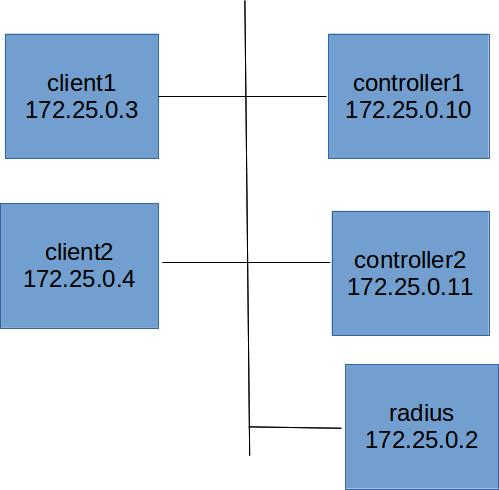
\includegraphics [width=0.8\textwidth]{radius.jpg}
\end{center}
\caption{Network topology for the Radius lab}
\label{fig:topology}
\end{figure}

\section{Lab Tasks}
\subsection{Explore}
Start wireshark on the radius server:
\begin{verbatim}
   wireshark &
\end{verbatim}
\noindent and select the eth0 interface and start capturing data.

Then start the radius service in debug mode:
\begin{verbatim}
    radiusd -X
\end{verbatim}

On client1, connect to controller1:
\begin{verbatim}
    ./control_admin controller1
\end{verbatim}
\noindent When prompted, provide {\tt hardcoded\_password} as the password.
\footnote{If the control\_admin program
repeatedly informs you that the password is not correct, that may be
due to the radius service not running.}
Observe the traffic in wireshark. 

Then use {\tt exit} to exit from controller1.  And now try to access
controller2, again using a password of: {\tt hardcoded\_password}
\begin{verbatim}
    ./control_admin controller2
\end{verbatim}
\noindent What do you observe at the radius service?  And in wireshark?

\subsection{Configure radius for controller2}
The controller2 device has been pre-configured to use your Radius server for 
authentication of users.  That means it has the shared secret used by Radius
to encrypt user passwords, and it knows the IP address of the radius server.
However, the Radius server is not configured to serve controller2.  You must
change the Radius server configuration to recognize controller2.
Use Ctrl-c at the radius server to stop the service.
Edit the {\tt /etc/raddb/clients.conf} file to allow controller2 to authenticate
via the radius service, and then restart the radius service.

Try again to access controller2 from one of the clients.

\subsection{Change the cadmin password}
Stop the radius service and edit the {\tt /etc/raddb/users} file to change the 
password of the cadmin user to something other than {\tt hardcoded\_password}.  Then test your abilty
use the config\_admin  utility to access the controllers with the new password.

\section{Submission}
After finishing the lab, go to the terminal on your Linux system that was used to start the lab and type:
\begin{verbatim}
    stoplab 
\end{verbatim}
When you stop the lab, the system will display a path to the zipped lab results on your Linux system.  Provide that file to 
your instructor, e.g., via the Sakai site.

\end{document}
